\chapter{Protocolli e demoni di sincronizzazione analizzati}
\label{cha:protocolliAndDemoni}

\section{Protocollo, implementazione e demone}

Prima di entrare nel dettaglio dei protocolli e implementazioni usate nell'attività
sperimentale, è utile chiarire la distinzione che vi è presente tra protocollo, implementazione
software e demone. Questi tre livelli sono collegati ma non coincidono.

Un protocollo di rete, in telecomunicazioni, è un particolare tipo di protocollo
di comunicazione preposto al funzionamento di una rete informatica ovvero la
definizione formale a priori delle modalità o regole di interazione che due o
più apparecchiature elettroniche collegate tra loro devono rispettare per
operare particolari funzionalità di elaborazione necessarie all'espletamento di
un certo servizio di rete.

In senso lato, un protocollo di comunicazione definisce la struttura ex ante, la
quale può essere adatta ad ogni sua possibile interpretazione attraverso l'implemntazione
pratica, delineando alla base le regole logiche dello scambio di messaggi, il
formato delle informazioni trasmesse, il modello di sincornizzazione e più in generale,
il comporamento atteso dai nodi coinvolte. \cite{ProtocolloDiRete2026}

L'implementazione software costituisce la parte pratica, ovvero la realizzazione concreta
di tali regole all'interno di un sistema operativo.

Infine un demone è un programma che viene eseguito come processo in background,
anziché essere sotto il controllo diretto di un utente interattivo
\cite{DaemonComputing2026}, nel caso specifico è responsabile dell'applivazione dell'alogritmo
di sincronizzazione e della gestione del clock locale.

Nel contesto della sincronizzazione temporale, i due protocolli presi ad esame
sono rispettivamente NTP e PTP. Network Time Protocol, definito nella sua
versione 4, dalla specifica \texttt{\textbf{RFC 5905}}. Precision Time Protocol definito
dallo standard \texttt{\textbf{IEEE 1588}}. È importante notare come la analisi sperimentale
che ne seguirà non deriva semplicemnte dalla differenza di protocollo utilizzato,
ma anche dalla sua implementazione plastica.

Per questa ragione, nella presente tesi vengono distinti i protocolli in riferimento
dagli strumenti software effettivamente analizzate. Nel dettaglio abbiamo NTPsec,
Chrony e linuxptp.

NTPsec e Chrony sono due distribuzioni che implmentano NTPv4 secondo RFC 5905,
derivate da NTP Classic, l'originale di Dave Mills, orientate a una
realizzazione più moderna e mantenibile del protocollo.\cite{SecureNetworkTime}.

Il servizio di sincronizzazione fornito da NTPsec viene eseguito tramite il
demone \texttt{ntpd}, cioè il processo che opera sul nodo e mantiene il clock
locale sincronizzato rispetto alle sorgenti configurate.

L'implementazione Chrony, una suite software alternativa di NTPsec, comprende
due programmi, il primo denominato \texttt{\textbf{chronyd}} è un demone che può
essere avviato all'avvio del sistema e chronyc è un programma con interfaccia a
command-line che può essere utilizzato per monitorare le prestazioni di chronyd
e per modificare vari parametri operativi mentre è in esecuzione. \cite{ChronyIntroduction}

Sebbene NTPsec e Chrony siano entrambi basati sul protocollo NTP, i rispettivi demoni
espongono le informazioni di sincronizzazione attraverso strutture e metriche non
completamente coincidenti. Alcune grandezze sono concettualmente analoghe, come offset,
delay, stratum e informazioni sulla raggiungibilità della sorgente; altre sono
specifiche del modo in cui ciascuna implementazione rappresenta lo stato del
clock, la qualità della sorgente e il processo interno di stima.

Nel caso di PTP, vi è una distinzione analoga ma rispetto ad uno standard
differente. L'implementazione software analizzata disponibile in ambiente linux è
rispettivamente \texttt{\textbf{linuxptp}}. In particolare, il demone
considerato è \texttt{\textbf{ptp4l}}.

La distinzione sopra riportata è fondamentale nel distinguere i diversi piani di comparazione
che ne seguiranno. Le metriche raccolte nel capitolo
\ref{cha:AnalisiSperimentale} descirivono quindi il comportamento concreto dei
demoni in questione nelle condizioni sperimentali definite, oltre alle ovvie proprietà
teoriche dei protocolli a cui essi si referiscono.

\section{Network Time Protocol}
\subsection{Caratteristiche generali}
Network Time Protocol (NTP) è uno dei principali protocolli di sincronizzazionte temporale
utilizzati in reti di computer. NTP è stato progettato per sincronizzare gli
orologi dei computer su Internet e su reti locali, garantendo che tutti i dispositivi
coinvolti abbiano un tempo coerente. La versione più recente di NTP è la
versione 4, definita nella specifica RFC 5905.

L'implementazione di NTP assume funzione di server primario, server secondario o client.
Un server primario è sincronizzato con un orologio di riferimento direttamente
riconducibile all'UTC (ad esempio, GPS, Galileo, ecc.). Un client si sincronizza con
uno o più server upstream, ma non fornisce la sincronizzazione ai client
dipendenti. Un server secondario ha uno o più server upstream e uno o più server downstream
o client. \cite{martinNetworkTimeProtocol2010}

\begin{figure}[H]
  \centering
  \begin{subfigure}
    {0.32\textwidth}
    \centering
    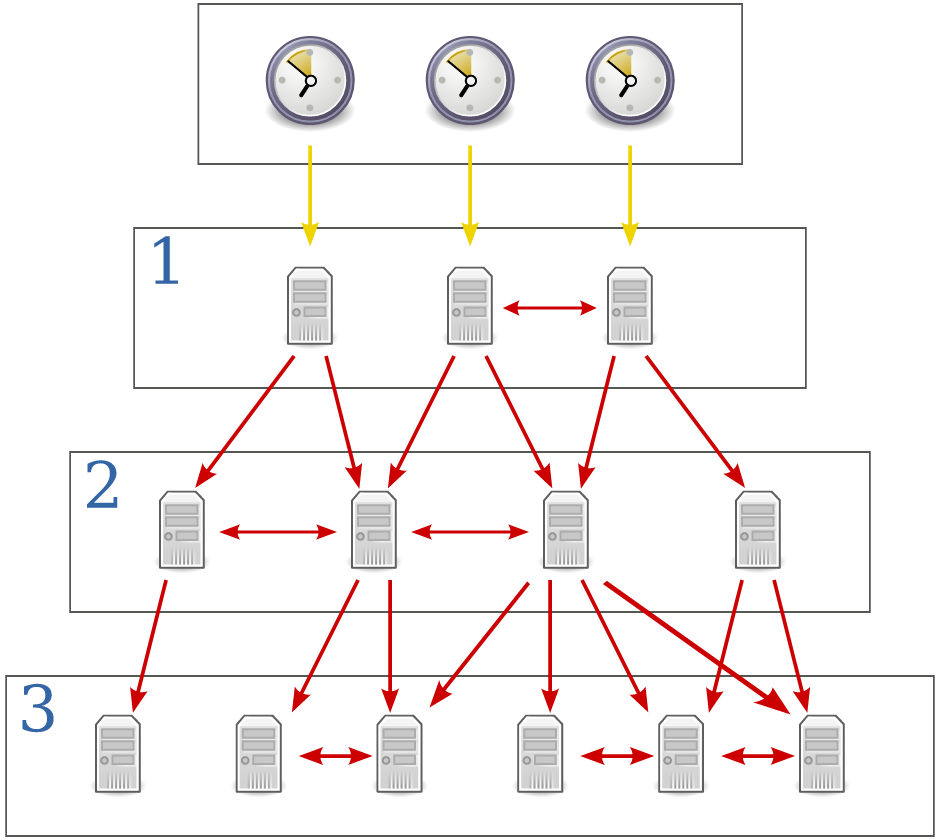
\includegraphics[width=\linewidth]{
      images/theory/Network_Time_Protocol_servers_and_clients.png
    }
    \caption{NTP hierarchy \cite{NetworkTimeProtocol2026}}
  \end{subfigure}
\end{figure}

Il protocollo generalmente opera sopra UDP, sulla porta 123, e utilizza lo
scambio di messaggi timestamp per stimare il ritardo di rete e l'offset tra il
clock locale e una sorgente temporale di riferimento.

\subsection{Modalità operative e topologia gerarchica}
Nella specifica vi sono tre varianti del protocollo NTP, rispettivamente simmetrico,
client/server e broadcast. Ognuna di queste varianti è associata a un diverso insieme
di modalità di pacchetto, che sono indicate in un campo specifico all'interno
del pacchetto NTP. \ref{tab:ntp_association_packet_modes}.

\begin{table}[h]
  \centering
  \begin{tabular}{lcc}
    \hline
    \textbf{Association Mode} & \textbf{Assoc. Mode Value} & \textbf{Packet Mode Value} \\
    \hline
    Symmetric Active          & 1                          & 1 or 2                     \\
    Symmetric Passive         & 2                          & 1                          \\
    Client                    & 3                          & 4                          \\
    Server                    & 4                          & 3                          \\
    Broadcast Server          & 5                          & 5                          \\
    Broadcast Client          & 6                          & N/A                        \\
    \hline
  \end{tabular}
  \caption{Association and packet modes in NTP.}
  \label{tab:ntp_association_packet_modes}
\end{table}

Nella v

Nella variante \texttt{client/server}, un client persistente invia pacchetti di modalità
4 a un server, che restituisce pacchetti di modalità 3. I server forniscono
sincronizzazione a uno o più client, ma non accettano sincronizzazione da loro.
Un server può anche essere un driver di orologio di riferimento che ottiene il
tempo direttamente da una fonte standard come un ricevitore GPS o un servizio di
modem telefonico. In questa variante,i client estraggono la sincronizzazione dai server.
Variante utilizzata in fase di testing, in entrambi le implementazioni NTPsec \ref{NTPsec}
e Chrony \ref{Chrony}.

Nella modalità \texttt{symmetric} due nodi operano come peer. Ciascun peer può trattare
l'altro come potenziale sorgente temporale e la relazione non è strutturata secondo
una direzione gerarchica client--server. Questa modalità è adatta a scenari in cui
più server temporali cooperano tra loro come nodi di pari livello.

La modalità \texttt{broadcast} prevede infine che un server invii periodicamente
messaggi temporali destinati a più client. I client possono ricevere passivamente
tali aggiornamenti, eventualmente dopo una fase iniziale di calibrazione del
ritardo. Questa modalità è utile quando si vuole distribuire la sincronizzazione a
più nodi riducendo lo scambio individuale di messaggi.

Il livello ricoperto da ciascun server nella gerarchia è definito secondo una numerazione
di stratum. Partendo da stratum 1, associato a server primari, si può arrivare
ad un massimo di 15 (16 si considera non sincronizzato). All'aumentare del numero
di stratum, la sua precisione si degrada a seconda del percorso di rete
specifico e della stabilità dell'orologio di sistema. Gli errori medi, misurati
in base alle distanze di sincronizzazione, aumentano approssimativamente in proporzione
ai numeri di stratum e al ritardo di andata e ritorno misurato.

NTP organizza la sincronizzazione secondo una struttura gerarchica orientata a evitare
cicli e a minimizzare la distanza di sincronizzazione rispetto alle sorgenti primarie.
La RFC 5905 descrive tale organizzazione come basata su una variante dell'algoritmo
distribuito Bellman-Ford, utilizzata per determinare uno spanning tree dei percorsi
più brevi radicato sui primary server~ \cite{martinNetworkTimeProtocol2010} In
questo modo, la subnet NTP può riorganizzarsi automaticamente in presenza di guasti
o variazioni nella rete temporale.

-------------
\subsection{Stima di offset e delay}
Il tempo di sistema è rappresentato dall'orologio di sistema gestito dall'hardware
e dal sistema operativo. L'obiettivo degli algoritmi NTP è minimizzare sia la
differenza di tempo che la differenza di frequenza tra UTC (Coordinated Universal
Time, o l'orologio di riferimento) e l'orologio di sistema. Quando queste
differenze sono state ridotte al di sotto delle tolleranze nominali, si dice che l'orologio
di sistema è sincronizzato con UTC. Un timestamp $T(t)$ rappresenta la data UTC
o l'offset di tempo rispetto a UTC al tempo di esecuzione t. Il significato inteso
dovrebbe essere chiaro dal contesto. Sia $T(t)$ l'offset di tempo, $R(t)$ l'offset
di frequenza e $D(t)$ il tasso di invecchiamento (derivata prima di $R(t)$
rispetto a t). Quindi, se $T(t_{0})$ è lo scostamento temporale UTC determinato a
$t = t_{0}$, lo scostamento temporale UTC al tempo t è

\[
  T(t) = T(t_{0}) + R(t_{0})(t-t_{0}) + 1/2 * D(t_{0})(t-t_{0})^{2}+ e
\]

dove e è un termine di errore stocastico.

Quattro statistiche vengono aggiornate ogni volta che un client effettua una
misurazione con un server. Lo scomostamento, ossia il \texttt{theta}, è
rappresentazione dello scostamento temporale di massima verosimiglianza dell'orologio
del server rispetto all'orologio di sistema. Vi è poi il ritardo,definito come \texttt{delta},
che è definito come il ritardo di andata e ritorno tra client e server. Vi è poi
la dispersione, \texttt{epsilon} cioè l'errore massimo intrinseco alla
misurazione, la quale aumenta a una velocità pari alla massima tolleranza di frequenza
dell'orologio di sistema disciplinato $PHI$, tipicamente 15 ppm. Infine, il
jitter, definito come \texttt{psi}, è la media quadratica (RMS) delle differenze di
offset più recenti e rappresenta l'errore nominale nella stima dell'offset.

La specifica NTPv4 descrive inoltre il protocollo come un insieme di processi e strutture
di stato, distinguendo tra variabili associate ai pacchetti, allo stato dei peer,
al processo di polling, allo stato di sistema e alla disciplina del clock \cite{martinNetworkTimeProtocol2010}.
Questa organizzazione evidenzia che il demone non si limita a ricevere timestamp
e applicare una correzione immediata, ma mantiene informazioni sullo stato delle associazioni,
valuta la qualità delle sorgenti e utilizza tali informazioni nel processo di
selezione, filtraggio e correzione del clock locale.

Dal punto di vista dei dati scambiati, un pacchetto NTP contiene informazioni
relative sia allo stato della sorgente temporale sia ai timestamp necessari alla
stima del tempo. Tra i campi più rilevanti per l'analisi della sincronizzazione vi
sono \texttt{mode}, che identifica la modalità del pacchetto, \texttt{stratum},
che indica la distanza gerarchica dalla sorgente di riferimento, \texttt{poll}, che
descrive l'intervallo di interrogazione, \texttt{rootdelay} e \texttt{rootdisp}, che
rappresentano rispettivamente il ritardo e la dispersione cumulativi verso la sorgente
primaria, e \texttt{refid}, che identifica il riferimento temporale utilizzato. Il
pacchetto include inoltre i timestamp \texttt{org}, \texttt{rec}, \texttt{xmt} e
\texttt{dst}, corrispondenti ai quattro istanti utilizzati nel modello di stima
di delay e offset. \cite{martinNetworkTimeProtocol2010}

Dal punto di vista del formato dei messaggi, un pacchetto NTP è trasportato come datagramma
UDP e contiene un header composto da campi che descrivono sia lo stato della sorgente
temporale sia i timestamp utilizzati per la stima della sincronizzazione \cite{martinNetworkTimeProtocol2010}.

Dal punto di vista del trasporto, NTP opera tramite pacchetti scambiati su UDP, tipicamente
sulla porta 123. La scelta di UDP è coerente con la natura della sincronizzazione
temporale: il protocollo non richiede consegna affidabile dei messaggi, poiché eventuali
ritrasmissioni introdurrebbero ulteriore ritardo e renderebbero meno rappresentativa
l'informazione temporale trasportata dal pacchetto. La RFC 5905 osserva infatti
che un trasporto affidabile, come TCP, può risultare controproducente per NTP, in
quanto i retry aumenterebbero il delay e gli errori associati alla stima temporale
\cite{martinNetworkTimeProtocol2010}.

Il protocollo on-wire si basa quindi sullo scambio di datagrammi contenenti timestamp
e informazioni di stato. Tali timestamp consentono di stimare il round-trip
delay e l'offset tra client e sorgente temporale. Ne consegue che la qualità della
sincronizzazione dipende direttamente dalle condizioni del percorso di rete:
delay variabile, jitter, perdita di pacchetti e congestione possono alterare la
regolarità delle osservazioni disponibili al demone.

\subsection{Filtraggio, selezione e disciplina del clock}
In NTPv4 è presente una sequenza di elaborazione delle osservazioni temporali, al
fine di ridurre l'effetto di misure rumorose, selezionare sorgenti coerenti e
correggere il clock del sistema in modo controllato
\cite{martinNetworkTimeProtocol2010}.

Il primo livello di elaborazione è il \textit{clock filter algorithm}. Per ogni
associazione con una sorgente temporale, il demone mantiene un insieme di campioni
recenti, ciascuno associato alle misure osservate. L'idea di base è individuare le
osservazioni più affidabili, privilegiando in generale campioni caratterizzati
da minore incertezza. In questo modo, il protocollo evita che una singola misura
degradata produca immediatamente una correzione errata del clock locale.

In seguito al filtraggio delle misure associate ai singoli peer, il demone procede
con il \textit{system process}, che valuta le sorgenti temporali disponibili.
Quando sono presenti più sorgenti, NTP deve stabilire quali siano coerenti tra loro
e quali debbano essere escluse perché considerate inaffidabili o anomale. Il
processo di selezione riduce quindi l'insieme delle sorgenti candidate e
individua il riferimento temporale da utilizzare per la sincronizzazione del
sistema. Anche quando nel testbed è presente una topologia controllata e con poche
sorgenti, questo meccanismo è concettualmente rilevante: la qualità della sorgente
percepita dal demone influenza lo stato operativo e le metriche riportate.

L'ultimo passaggio è la \textit{clock discipline}, cioè il meccanismo mediante il
quale le stime selezionate vengono utilizzate per correggere il clock locale. La
correzione non coincide necessariamente con uno spostamento immediato dell'orologio
di sistema. Il demone può intervenire anche regolando progressivamente la frequenza
di avanzamento del clock, in modo da ridurre l'offset preservando la continuità
temporale. Questa distinzione è importante: una misura di offset rappresenta una
stima dello scostamento, mentre la disciplina del clock determina come tale stima
viene trasformata in una correzione effettiva.

\subsection{NTPsec e il demone ntpd}

NTPsec è un progetto nato con l'obiettivo di fornire una implementazione più
sicura e manutenibile del protocollo NTP, mantenendo la compatibilità con la specifica
RFC 5905. Il progetto si è sviluppato a partire da NTP Classic. L'obiettivo di
NTPsec è quello di offrire una versione più robusta e semplificata del
protocollo, ottenutos anche attraverso la rimozione di codice legacy e funzionalità
obsolete. Questa caratteristica è rilevante soprattutto in contesti in cui il
demone di sincronizzazione è esposto in rete e deve operare come componente
infrastrutturale affidabile \cite{SecureNetworkTime}.

Il componente principale della suite è il demone \texttt{ntpd}, responsabile
dell'esecuzione del servizio NTP sul nodo. Il demone gestisce le associazioni configurate,
comunica con le sorgenti temporali, mantiene lo stato della sincronizzazione e applica
le correzioni necessarie al clock locale. Accanto al demone, la suite fornisce strumenti
di interrogazione e controllo, come \texttt{ntpq}, utilizzabili per osservare lo
stato delle associazioni e le metriche prodotte dal servizio.

\begin{table}[h]
  \centering
  \begin{tabular}{lll}
    \hline
    \textbf{Comando / fonte} & \textbf{Metrica / campo}       & \textbf{Significato}                                           \\
    \hline
    \texttt{ntpq -p}         & \texttt{remote}                & Sorgente o peer NTP remoto configurato.                        \\
    \texttt{ntpq -p}         & \texttt{refid}                 & Identificativo della sorgente temporale di riferimento.        \\
    \texttt{ntpq -p}         & \texttt{st}                    & Stratum della sorgente remota.                                 \\
    \texttt{ntpq -p}         & \texttt{t}                     & Tipo di associazione NTP.                                      \\
    \texttt{ntpq -p}         & \texttt{when}                  & Tempo trascorso dall'ultimo pacchetto ricevuto dalla sorgente. \\
    \texttt{ntpq -p}         & \texttt{poll}                  & Intervallo di polling verso la sorgente.                       \\
    \texttt{ntpq -p}         & \texttt{reach}                 & Registro di raggiungibilità della sorgente.                    \\
    \texttt{ntpq -p}         & \texttt{delay}                 & Ritardo stimato del percorso verso la sorgente.                \\
    \texttt{ntpq -p}         & \texttt{offset}                & Scostamento stimato tra clock locale e sorgente temporale.     \\
    \texttt{ntpq -p}         & \texttt{jitter}                & Variabilità delle misure associate alla sorgente.              \\
    \hline
    \texttt{peerstats}       & \texttt{offset}                & Scostamento stimato rispetto al peer remoto.                   \\
    \texttt{peerstats}       & \texttt{delay}                 & Ritardo stimato dell'associazione con il peer.                 \\
    \texttt{peerstats}       & \texttt{dispersion}            & Incertezza stimata della misura temporale.                     \\
    \texttt{peerstats}       & \texttt{jitter}                & Jitter RMS associato alle misure del peer.                     \\
    \hline
    \texttt{loopstats}       & \texttt{offset}                & Offset del clock locale rispetto alla sorgente selezionata.    \\
    \texttt{loopstats}       & \texttt{frequency}             & Correzione di frequenza applicata al clock locale.             \\
    \texttt{loopstats}       & \texttt{jitter}                & Variabilità stimata del clock locale.                          \\
    \texttt{loopstats}       & \texttt{wander}                & Variabilità lenta della frequenza del clock locale.            \\
    \hline
    \texttt{rawstats}        & \texttt{originate timestamp}   & Timestamp di invio della richiesta da parte del client.        \\
    \texttt{rawstats}        & \texttt{receive timestamp}     & Timestamp di ricezione della richiesta presso il server.       \\
    \texttt{rawstats}        & \texttt{transmit timestamp}    & Timestamp di invio della risposta da parte del server.         \\
    \texttt{rawstats}        & \texttt{destination timestamp} & Timestamp locale di ricezione della risposta presso il client. \\
    \hline
    \texttt{readvar}         & \texttt{rootdelay}             & Ritardo cumulativo verso la sorgente primaria.                 \\
    \texttt{readvar}         & \texttt{rootdisp}              & Dispersione cumulativa verso la sorgente primaria.             \\
    \texttt{readvar}         & \texttt{stratum}               & Livello gerarchico del sistema locale.                         \\
    \texttt{readvar}         & \texttt{refid}                 & Identificativo della sorgente selezionata.                     \\
    \texttt{readvar}         & \texttt{leap}                  & Stato relativo alla sincronizzazione e ai leap second.         \\
    \hline
  \end{tabular}
  \caption{Principali metriche e campi esposti da NTPsec tramite \texttt{ntpd},
  \texttt{ntpq} e file statistici, rielaborati dalla documentazione ufficiale~\cite{ntpsec-doc}.}
  \label{tab:ntpsec_metriche}
\end{table}

\subsection{Chrony e il demone chronyd}
\label{Chrony}

Chrony è una suite software per la sincronizzazione temporale e costituisce una
implementazione versatile del Network Time Protocol. Il progetto è progettato per
sincronizzare il clock di sistema rispetto a server NTP, reference clock, come ricevitori
GPS, oppure input manuali; può inoltre operare come server NTPv4, fornendo
sincronizzazione ad altri nodi della rete~\cite{ChronyDocumentation}.

Dal punto di vista protocollare, Chrony non definisce un protocollo alternativo a
NTP, ma implementa la sincronizzazione basata su NTP con una propria
architettura software e proprie strategie interne di stima e controllo del clock.
Questa distinzione è rilevante nel contesto della tesi, poiché Chrony e NTPsec
appartengono allo stesso ambito protocollare, ma rappresentano implementazioni differenti:
eventuali differenze di comportamento devono quindi essere ricondotte non al
protocollo di riferimento, bensì alle scelte implementative e operative dei rispettivi
demoni.

La suite Chrony è composta principalmente da due programmi: \texttt{chronyd} e \texttt{chronyc}.
Il primo è il demone responsabile della sincronizzazione del clock locale e viene
normalmente eseguito come servizio di sistema. Il secondo è un'interfaccia a
riga di comando che consente di interrogare lo stato del demone, monitorarne le prestazioni
e modificare alcuni parametri operativi durante l'esecuzione \cite{ChronyDocumentation}.

Una caratteristica rilevante di Chrony è la sua progettazione orientata al funzionamento
in condizioni operative variabili. La documentazione del progetto evidenzia
infatti il supporto a scenari quali connessioni di rete intermittenti, reti congestionate,
variazioni di temperatura che influenzano il clock locale, sistemi non sempre attivi
e ambienti virtualizzati \cite{ChronyDocumentation}. Queste caratteristiche
rendono Chrony particolarmente adatto a contesti nei quali la sincronizzazione
deve rimanere efficace anche quando la disponibilità della sorgente temporale o
la qualità del percorso di rete non sono costanti.

Le metriche rese disponibili da Chrony, in particolare attraverso le informazioni
di \textit{tracking} e \textit{sourcestats}, permettono di osservare lo stato
del clock locale, la qualità della sorgente temporale e la variabilità delle misure
utilizzate dal demone.

\begin{table}[h]
  \centering
  \begin{tabular}{lll}
    \hline
    \textbf{Comando / fonte} & \textbf{Metrica / campo} & \textbf{Significato}                                                         \\
    \hline
    \texttt{tracking}        & \texttt{Reference ID}    & Identificativo della sorgente selezionata.                                   \\
    \texttt{tracking}        & \texttt{Stratum}         & Livello gerarchico del nodo rispetto alla sorgente primaria.                 \\
    \texttt{tracking}        & \texttt{Ref time}        & Istante dell'ultimo aggiornamento dal riferimento.                           \\
    \texttt{tracking}        & \texttt{System time}     & Scostamento residuo del clock di sistema rispetto al tempo stimato corretto. \\
    \texttt{tracking}        & \texttt{Last offset}     & Ultimo offset misurato rispetto alla sorgente selezionata.                   \\
    \texttt{tracking}        & \texttt{RMS offset}      & Valore quadratico medio degli offset recenti.                                \\
    \texttt{tracking}        & \texttt{Frequency}       & Correzione di frequenza applicata al clock locale.                           \\
    \texttt{tracking}        & \texttt{Residual freq}   & Frequenza residua stimata dopo la correzione.                                \\
    \texttt{tracking}        & \texttt{Skew}            & Incertezza nella stima della frequenza del clock.                            \\
    \texttt{tracking}        & \texttt{Root delay}      & Ritardo cumulativo verso la sorgente primaria.                               \\
    \texttt{tracking}        & \texttt{Root dispersion} & Dispersione cumulativa verso la sorgente primaria.                           \\
    \texttt{tracking}        & \texttt{Update interval} & Intervallo tra gli ultimi aggiornamenti della sincronizzazione.              \\
    \texttt{tracking}        & \texttt{Leap status}     & Stato relativo alla sincronizzazione e ai leap second.                       \\
    \hline
    \texttt{sources}         & \texttt{MS}              & Tipo e stato della sorgente temporale.                                       \\
    \texttt{sources}         & \texttt{Name/IP address} & Nome o indirizzo della sorgente.                                             \\
    \texttt{sources}         & \texttt{Stratum}         & Stratum dichiarato dalla sorgente.                                           \\
    \texttt{sources}         & \texttt{Poll}            & Intervallo di polling verso la sorgente.                                     \\
    \texttt{sources}         & \texttt{Reach}           & Registro di raggiungibilità della sorgente.                                  \\
    \texttt{sources}         & \texttt{LastRx}          & Tempo trascorso dall'ultimo campione ricevuto.                               \\
    \texttt{sources}         & \texttt{Last sample}     & Ultimo offset misurato rispetto alla sorgente.                               \\
    \hline
    \texttt{sourcestats}     & \texttt{NP}              & Numero di campioni mantenuti per la sorgente.                                \\
    \texttt{sourcestats}     & \texttt{NR}              & Numero di run dei residui con lo stesso segno.                               \\
    \texttt{sourcestats}     & \texttt{Span}            & Intervallo temporale coperto dai campioni.                                   \\
    \texttt{sourcestats}     & \texttt{Frequency}       & Frequenza stimata rispetto alla sorgente.                                    \\
    \texttt{sourcestats}     & \texttt{Freq Skew}       & Incertezza della stima di frequenza.                                         \\
    \texttt{sourcestats}     & \texttt{Offset}          & Offset stimato della sorgente.                                               \\
    \texttt{sourcestats}     & \texttt{Std Dev}         & Deviazione standard dei residui delle misure.                                \\
    \hline
  \end{tabular}
  \caption{Principali metriche e campi esposti da Chrony tramite \texttt{chronyc}.}
  \label{tab:chrony_metriche}
\end{table}

\section{Precision Time Protocol}
\subsection{Caratteristiche generali di PTP}
\subsection{linuxptp e il demone ptp4l}

\section{Motivazione della scelta degli strumenti analizzati}